\documentclass[letterpaper, 11pt, notitlepage]{report}

% --- Main packages ---

\usepackage[dvipsnames]{xcolor} % Extended set of colors

\usepackage{
  amsmath, amsthm, amssymb, mathtools, dsfont, units, % Math typesetting
  graphicx, wrapfig, subfig, float, % Figures and graphics formatting
  listings, color, inconsolata, pythonhighlight, % Code formatting
  fancyhdr, sectsty, hyperref, enumerate, enumitem, framed } % Headers/footers, section fonts, links, lists

\usepackage{hyperref} 

\usepackage{newpxtext, newpxmath, inconsolata} % Fonts

% --- Page layout settings ---

% Set page margins
\usepackage[left=1.35in, right=1.35in, top=1.0in, bottom=.9in, headsep=.2in, footskip=0.35in]{geometry}

% Anchor footnotes to the bottom of the page
\usepackage[bottom]{footmisc}

% Set line spacing
\renewcommand{\baselinestretch}{1.2}

% Set spacing between paragraphs
\setlength{\parskip}{1.3mm}

% Allow multi-line equations to break onto the next page
\allowdisplaybreaks

% --- Page formatting settings ---

% Set image captions to be italicized
\usepackage[font={it,footnotesize}]{caption}

% Set link colors for labeled items (blue), citations (red), URLs (orange)
\hypersetup{colorlinks=true, linkcolor=RoyalBlue, citecolor=RedOrange, urlcolor=ForestGreen}

% Set font size for section titles (\large) and subtitles (\normalsize) 
\usepackage{titlesec}
\usepackage{adforn}

\definecolor{gray75}{gray}{0.75}
\newcommand{\hsp}{\hspace{10pt}}

\titleformat{\chapter}{\LARGE\bfseries}{{\fontsize{22}{0}\selectfont\thechapter\hsp\textcolor{gray75}{|}\hsp}\;\;}{0em}{}
\titleformat{\section}{\Large\bfseries}{{\fontsize{15}{0}\selectfont\thesection}\;\;}{0em}{}
\titleformat{\subsection}{\normalsize\bfseries\selectfont}{{\fontsize{12}{16}\selectfont\adfoutlineleafright}\;\;}{0em}{}

% Enumerated/bulleted lists: make numbers/bullets flush left
%\setlist[enumerate]{wide=2pt, leftmargin=16pt, labelwidth=0pt}
\setlist[itemize]{wide=0pt, leftmargin=15pt, labelwidth=1pt, align=left, itemsep=0pt}

% --- Table of contents settings ---

\setcounter{tocdepth}{1} 
\usepackage[subfigure]{tocloft}

% Reduce spacing between sections in table of contents
\setlength{\cftbeforesecskip}{.9ex}

% Remove indentation for sections
%\cftsetindents{chapter}{0em}{10em}
%\cftsetindents{section}{0em}{10em}

% Set font size (\large) for table of contents title
\renewcommand{\cfttoctitlefont}{\large\bfseries}

% Remove numbers/bullets from section titles in table of contents
%\makeatletter
%\renewcommand{\cftsecpresnum}{\begin{lrbox}{\@tempboxa}}
%\renewcommand{\cftsecaftersnum}{\end{lrbox}}
%\makeatother
%
%\makeatletter
%\renewcommand{\cftchappresnum}{\begin{lrbox}{\@tempboxa}}
%\renewcommand{\cftchapaftersnum}{\end{lrbox}}
%\makeatother

% --- Math/Statistics commands ---

% Add a reference number to a single line of a multi-line equation
% Usage: "\numberthis\label{labelNameHere}" in an align or gather environment
\newcommand\numberthis{\addtocounter{equation}{1}\tag{\theequation}}

% Shortcut for bold text in math mode, e.g. $\b{X}$
\let\b\mathbf

% Shortcut for bold Greek letters, e.g. $\bg{\beta}$
\let\bg\boldsymbol

% Shortcut for calligraphic script, e.g. %\mc{M}$
\let\mc\mathcal

% --- Left/right header text (to appear on every page) ---

% Do not include a line under header or above footer
\pagestyle{fancy}
\renewcommand{\footrulewidth}{0pt}
\renewcommand{\headrulewidth}{0pt}

% Right header text: Lecture number and title
\renewcommand{\sectionmark}[1]{\markright{#1} }
\fancyhead[R]{\small\textit{\nouppercase{\rightmark}}}

% Left header text: Short course title, hyperlinked to table of contents
\fancyhead[L]{\hyperref[sec:contents]{\small HE-AP Th}}

% Add bibliography to TOC
\usepackage[nottoc,numbib]{tocbibind}

\usepackage{amsmath,amsthm,amsfonts,amssymb,amscd}
\usepackage{aas_macros}
\usepackage{booktabs}
%\usepackage{calc}
\usepackage{cancel}
%\usepackage{empheq}
%\usepackage{enumitem}
%\usepackage{fancyhdr}
%\usepackage{framed}
%\usepackage{fullpage}
%\usepackage[margin=3cm]{geometry}
%\usepackage[utf8]{inputenc}
%\usepackage{lastpage}
%\usepackage{mathabx}
%\usepackage{mathrsfs}
%\usepackage{mdframed}
%\usepackage{multicol}
%\usepackage{multirow}
\usepackage{physics}
%\usepackage{setspace}
%\usepackage[most]{tcolorbox}
%\usepackage{todonotes}
%\usepackage{wrapfig}
%%\usepackage[table]{xcolor}
%
%\newlength{\tabcont}
\setlength{\parindent}{0.0in}
\setlength{\parskip}{0.05in}
%\colorlet{shadecolor}{orange!15}
%\parindent 0in
%\parskip 12pt
%\geometry{margin=1in, headsep=0.25in}
%
%\theoremstyle{definition}
%\newtheorem{defn}{Definition}
%\newtheorem{reg}{Rule}
%\newtheorem{exer}{Exercise}
%\newtheorem{note}{Note}
%\newtheorem{tbd}{Demonstration}
%
%\linespread{1.1}
%
%\usepackage{sectsty}
%\sectionfont{\large}
%
%\usepackage{hyperref}
%\hypersetup{
%    colorlinks,
%    citecolor=red,
%    filecolor=red,
%    linkcolor=blue,
%    urlcolor=red
%}

\newcommand\drsh{\rotatebox[origin=c]{180}{$\Lsh$}}

\DeclareRobustCommand{\rchi}{{\mathpalette\irchi\relax}}
\newcommand{\irchi}[2]{\raisebox{\depth}{$#1\chi$}} 

% theorems
\makeatother
\usepackage{thmtools}
\usepackage[framemethod=TikZ]{mdframed}
\mdfsetup{skipabove=1em,skipbelow=0em}

\theoremstyle{definition}

%\declaretheoremstyle[
%    headfont=\bfseries\sffamily\color{ForestGreen!70!black}, bodyfont=\normalfont,
%    mdframed={
%        linewidth=2pt,
%        rightline=false, topline=false, bottomline=false,
%        linecolor=ForestGreen, backgroundcolor=ForestGreen!5,
%    }
%]{thmgreenbox}

\declaretheoremstyle[
    headfont=\bfseries\sffamily\color{Red!70!black}, bodyfont=\normalfont,
    mdframed={
        linewidth=2pt,
        rightline=false, topline=false, bottomline=false,
        linecolor=Red, backgroundcolor=Red!5,
    }
]{thmredbox}

\declaretheoremstyle[
    headfont=\bfseries\sffamily\color{NavyBlue!70!black}, bodyfont=\normalfont,
    mdframed={
        linewidth=2pt,
        rightline=false, topline=false, bottomline=false,
        linecolor=NavyBlue, backgroundcolor=NavyBlue!5,
    }
]{thmbluebox}

\declaretheoremstyle[
    headfont=\bfseries\sffamily\color{NavyBlue!70!black}, bodyfont=\normalfont,
    mdframed={
        linewidth=2pt,
        rightline=false, topline=false, bottomline=false,
        linecolor=NavyBlue
    }
]{thmblueline}

%\declaretheoremstyle[
%    headfont=\bfseries\sffamily\color{RawSienna!70!black}, bodyfont=\normalfont,
%    mdframed={
%        linewidth=2pt,
%        rightline=false, topline=false, bottomline=false,
%        linecolor=RawSienna, backgroundcolor=RawSienna!5,
%    }
%]{thmredbox}
%
%\declaretheoremstyle[
%    headfont=\bfseries\sffamily\color{RawSienna!70!black}, bodyfont=\normalfont,
%    numbered=no,
%    mdframed={
%        linewidth=2pt,
%        rightline=false, topline=false, bottomline=false,
%        linecolor=RawSienna, backgroundcolor=RawSienna!1,
%    },
%    qed=\qedsymbol
%]{thmproofbox}
%
%\declaretheoremstyle[
%    headfont=\bfseries\sffamily\color{NavyBlue!70!black}, bodyfont=\normalfont,
%    numbered=no,
%    mdframed={
%        linewidth=2pt,
%        rightline=false, topline=false, bottomline=false,
%        linecolor=NavyBlue, backgroundcolor=NavyBlue!1,
%    },
%]{thmexplanationbox}

%\declaretheorem[style=thmgreenbox, name=Definition]{definition}
\declaretheorem[style=thmbluebox, numbered=no, name=Exercise]{exercise}
\declaretheorem[style=thmredbox, numbered=no, name=Solution]{solution}
%\declaretheorem[style=thmredbox, name=Proposition]{prop}
%\declaretheorem[style=thmredbox, name=Theorem]{theorem}
%\declaretheorem[style=thmredbox, name=Lemma]{lemma}
%\declaretheorem[style=thmredbox, numbered=no, name=Corollary]{corollary}

%\declaretheorem[style=thmproofbox, name=Proof]{replacementproof}
%\renewenvironment{proof}[1][\proofname]{\vspace{-10pt}\begin{replacementproof}}{\end{replacementproof}}

%\declaretheorem[style=thmexplanationbox, name=Proof]{tmpexplanation}
%\newenvironment{explanation}[1][]{\vspace{-10pt}\begin{tmpexplanation}}{\end{tmpexplanation}}
%\declaretheorem[style=thmredbox, numbered=no]{remark}

\newmdenv[  
topline=false,  
rightline=false,  
bottomline=false,  
leftline=true,  
linecolor=RawSienna!95!black,  
linewidth=3pt,  
backgroundcolor=RawSienna!10,  
]{remark} 

\declaretheorem[style=thmblueline, numbered=no, name=Note]{note}

% new \oset macro:
\makeatletter
\newcommand{\oset}[3][1.4ex]{%
  \mathrel{\mathop{#3}\limits^{
    \vbox to#1{\kern-2\ex@
    \hbox{$\scriptstyle#2$}\vss}}}}
\makeatother

%\newtheorem*{uovt}{UOVT}
%\newtheorem*{notation}{Notation}
%\newtheorem*{previouslyseen}{As previously seen}
%\newtheorem*{problem}{Problem}
%\newtheorem*{observe}{Observe}
%\newtheorem*{property}{Property}
%\newtheorem*{intuition}{Intuition}

\newcommand{\TODO}[1]{{\color{yellow!70!black}[#1]}}

\graphicspath{{figures/}{../figures/}}

\begin{document}

\title{High-Energy Astroparticle Theory \\[1em]
\normalsize A.Y.~2024/25}

\author{\normalsize Carmelo Evoli}
\date{\normalsize\vspace{-1ex} Last updated: \today}

\maketitle

\vspace{0.25cm}
{\color{red}\large This document is currently under active development. The content is subject to change as revisions are ongoing. I expect to release a stable and comprehensive version no earlier than January 2026.}
\vspace{0.25cm}

These lecture notes are largely based on:
%
\begin{itemize}
\item P.~Blasi, \emph{The origin of galactic cosmic rays}, A\&AR, 21, 70, 2013, \href{https://arxiv.org/abs/1311.7346}{arXiv:1311.7346}
\item P.D.~Serpico, \emph{Cosmic ray interactions with matter and radiation}, Proceedings of the International School of Physics ``Enrico Fermi'', Course 208, Varenna 2022, \href{https://arxiv.org/abs/2308.04361}{arXiv:2308.04361}
\item D.~Boncioli, \emph{Cosmic-ray propagation in extragalactic space and secondary messengers}, Proceedings of the International School of Physics ``Enrico Fermi'', Course 208, Varenna 2022, \href{https://arxiv.org/abs/2309.12743}{arXiv:2309.12743}
\item C.~Evoli \& U.~Dupletsa, \emph{Phenomenological models of Cosmic Ray transport in Galaxies}, Proceedings of the International School of Physics ``Enrico Fermi'', Course 208, Varenna 2022, \href{https://arxiv.org/abs/2309.00298}{arXiv:2309.00298}
\end{itemize}

Useful readings:
%
\begin{itemize}
\item M.~Vietri, \emph{Foundations of High-Energy Astrophysics}, April 2008, U.~Chicago Press
\item R.~Blandford \& D.~Eichler, \emph{Particle acceleration at astrophysical shocks: A theory of cosmic ray origin},  October 1987, Physics Reports, 154
\item G.B.~Rybicki \& A.P.~Lightman, \emph{Radiative Processes in Astrophysics}, May 1985, Vch Pub
\item T.K.~Gaisser, R.~Engel \& E.~Resconi, \emph{Cosmic Rays and Particle Physics}, June 2016, Cambridge University Press
\item D.~Overbye, \emph{Lonely Hearts of the Cosmos: The Story of the Scientific Quest for the Secret of the Universe}, November 1999, Back Bay Books
\end{itemize}

\newpage

\tableofcontents\label{sec:contents}

%\chapter{Radiative Processes in Astroparticle Physics}
%\input{sections/radiative/intro}
%\input{sections/radiative/synchrotron}
%\input{sections/radiative/inversecompton}
%\input{sections/radiative/gammaabsorption}
%\input{sections/radiative/hadronic}
%\newpage

\chapter{A Primer on Plasma Astrophysics}
%\input{sections/plasma/idealmhd}
%\input{sections/plasma/mhdwaves}
% !TEX root = ../../lectures.tex
%Awesome—your slides are spot-on in spirit: “bend the frozen-in field → magnetic tension pulls back,” exactly like a vibrating string. Below is the detailed, nuts-and-bolts derivation that makes the analogy precise and explains why the Alfvén speed follows the “(tension)/(linear density)” rule (actually (v^2=T/\mu)). I’ll also map each step to what you sketched in the slides. 

\section{Alfven waves in a mechanical analogy}

Start with a uniform plasma at rest with a uniform background field \(\mathbf B_0\). In ideal MHD, the field is \emph{frozen} into the plasma, so if you nudge a fluid element sideways to \(\mathbf B_0\), you bend the field lines. That bend stores magnetic energy, and the field develops a \emph{tension} that tries to straighten the lines, pushing the plasma back — this is the restoring force that launches a wave along \(\mathbf B_0\). 

%# 2) Magnetic tension from Maxwell stress (why there is a “tension”)

The magnetic force density can be written as
\[
\mathbf f = \underbrace{\frac{1}{4\pi}(\mathbf B\cdot\nabla)\mathbf B}_{\text{\tiny magnetic tension}} \underbrace{- \nabla\!\left(\frac{B^2}{8\pi}\right)}_{\text{\tiny gradient of magnetic pressure}}~.
\]
The second term is the \emph{magnetic pressure} (perpendicular squeezing), the first is the \emph{magnetic tension} (pulling \emph{along} field lines). When a field line is curved with radius of curvature (R), the tension produces a sideways restoring force
\[
f_{\perp} \sim \frac{B_0^2}{4\pi} \, \frac{1}{R}.
\]
This is the magnetic analog of a taut string that resists curvature.

%# 3) Reduce to a “string” (flux-tube) model

%Consider a thin flux tube of cross-section (A), mass density (\rho), and let (s) be the coordinate along the unperturbed field ((\hat{\mathbf b}*0\parallel\mathbf B_0)). Give it a small transverse displacement (\xi*\perp(s,t)) (say, in (y)). For small deflections, the curvature is (\kappa \approx \partial^2\xi_\perp/\partial s^2). The **total tension force** on a short segment of length (\Delta s) is then
%\[
%F_\perp ;=; \bigg(\frac{B_0^2}{4\pi}\bigg)A;\frac{\partial^2\xi_\perp}{\partial s^2},\Delta s,
%\]
%because the “tension per unit area along the field” is (B_0^2/4\pi) (cgs), and the geometric factor (\partial^2\xi_\perp/\partial s^2) measures how much the tension vectors at the two ends fail to cancel.
%
%\end{document}
%
%The **mass** of the segment is (\rho,A,\Delta s), so Newton’s 2nd law gives
%[
%\rho A,\Delta s;\frac{\partial^2\xi_\perp}{\partial t^2}
%;=;
%\bigg(\frac{B_0^2}{4\pi}\bigg)A;\frac{\partial^2\xi_\perp}{\partial s^2},\Delta s.
%]
%Cancel (A\Delta s) to obtain the transverse wave equation
%[
%\frac{\partial^2\xi_\perp}{\partial t^2}
%;=;
%\frac{B_0^2}{4\pi \rho},\frac{\partial^2\xi_\perp}{\partial s^2}.
%]

%# 4) Identify (T) and (\mu) → the “string formula”

Compare now with the standard string equation 
\( \partial_t^2 \xi = (T/\mu),\partial_s^2\xi \).
You can read off:
%
\begin{description}
\item[Tension] \(T = (B_0^2/4\pi),A \) — the magnetic tension times the tube area.
\item[Linear mass density] \(\mu = \rho,A\).
\end{description}

Therefore
\[
v_A^2 ;=; \frac{T}{\mu} ;=; \frac{B_0^2}{4\pi\rho}
\qquad\Rightarrow\qquad
\boxed{,v_A=\frac{B_0}{\sqrt{4\pi\rho}},}\quad\text{(cgs)}.
\]
%In SI units the same reasoning gives (v_A=B_0/\sqrt{\mu_0\rho}) because (B^2/4\pi) (cgs) ↔ (B^2/\mu_0) (SI). 

This is exactly the “tension over linear density” rule in your slide (with the square understood: \(c_w^2=T/\mu)\). 

Why propagation is \emph{along} \(\mathbf B_0\) only?

The restoring force comes from \emph{field-line curvature}, so the wave \emph{needs} variation along (s) (the direction of \(\mathbf B_0)\). 
%
If \(k_\parallel=0 \), there’s no curvature, hence no tension restoring force $\rightarrow$ no Alfvén propagation. That yields the dispersion
\[
\omega = \pm k_\parallel v_A,
\]
as you noted on the slide. 

Energy perspective (what’s doing “work”)

Bending the tube increases magnetic energy (magnetic pressure is unchanged to leading order for a pure Alfvén mode; it’s the **tension** piece that matters). During oscillation, magnetic energy and kinetic energy exchange and are equal on average—again matching the lossless string picture you referenced (“kinetic energy” ↔ “field-line bending”). 

Back to your numbers/remarks

%Your slide’s ISM estimate (v_A \simeq B/\sqrt{4\pi\rho_i}) (taking the ion mass density) and the remark that SNR shocks are super-Alfvénic, (v_{\rm SNR}\gg v_A), are exactly the standard scalings. With (B\sim \mathrm{few},\mu\mathrm G) and (n\sim 0.1\text{–}1,\mathrm{cm^{-3}}), one gets (v_A) of order (10\text{–}20,\mathrm{km,s^{-1}}), far below typical SNR shock speeds and of course (\ll c), as you wrote. 

\section{A primer on Alfven waves}

\subsection{Alfv\'en Waves (vs.\ Sound Waves)}

\paragraph{Setting and assumptions.}
We work in (ideal) MHD with a uniform equilibrium:
\[
\mathbf{B}_0=\text{const},\qquad \rho_0=\text{const},\qquad \mathbf{v}_0=\mathbf{0},\qquad p_0=\text{const}.
\]
Small perturbations $\delta \rho,\,\delta p,\,\delta \mathbf{v},\,\delta \mathbf{B}$ vary as $\exp[i(\mathbf{k}\!\cdot\!\mathbf{x}-\omega t)]$.
The ideal MHD equations we linearize are
\[
\begin{aligned}
&\partial_t \rho + \nabla\!\cdot(\rho \mathbf{v}) = 0,\\
&\rho\,\partial_t \mathbf{v} = -\nabla p + \frac{1}{\mu_0}(\nabla\times \mathbf{B})\times \mathbf{B},\\
&\partial_t \mathbf{B} = \nabla\times(\mathbf{v}\times \mathbf{B}),\qquad \nabla\!\cdot\!\mathbf{B}=0,\\
&\delta p = c_s^2\,\delta \rho\quad(\text{adiabatic closure, }c_s^2=\gamma p_0/\rho_0).
\end{aligned}
\]

\paragraph{Alfv\'en waves: definition and dispersion.}
Alfv\'en waves are \emph{transverse, incompressible} MHD waves whose restoring force is the magnetic tension of the background field $\mathbf{B}_0$.
They satisfy
\[
\delta \rho = 0,\qquad \delta p = 0,\qquad \mathbf{k}\cdot \delta\mathbf{v}=0,
\]
with polarization $\delta\mathbf{v}\perp\mathbf{B}_0$ and $\delta\mathbf{B}\perp\mathbf{B}_0$.
Writing $\mathbf{k}=k_\parallel \hat{\mathbf{b}}_0 + \mathbf{k}_\perp$ with $\hat{\mathbf{b}}_0=\mathbf{B}_0/B_0$, the dispersion relation is
\[
\boxed{\ \omega = \pm k_\parallel v_A\ ,\qquad v_A=\frac{B_0}{\sqrt{\mu_0 \rho_0}}\ } \quad
\text{(SI)}\qquad\text{or}\qquad v_A=\frac{B_0}{\sqrt{4\pi \rho_0}}\ \text{(cgs)}.
\]
Key features:
\begin{itemize}
\item Propagate \emph{along field lines}: no propagation if $k_\parallel=0$.
\item \emph{Transverse} polarization: $\delta\mathbf{v}\perp \mathbf{k}$ and $\delta\mathbf{v}\perp \mathbf{B}_0$ (shear Alfv\'en mode).
\item \emph{Incompressible}: no density/pressure perturbations at leading order.
\item Energy equipartition in linear waves: kinetic and magnetic perturbation energies are equal on average.
\item Group and phase velocities are $\pm v_A\,\hat{\mathbf{b}}_0$ (purely along $\mathbf{B}_0$).
\end{itemize}

\paragraph{Physical picture.}
Imagine a taut magnetic ``string'' (field line). A sideways displacement bends it, creating curvature and a \emph{tension} force $\propto B_0^2$ that pulls the plasma back; inertia is provided by $\rho_0$. The wave speed therefore scales as $v_A\propto B_0/\sqrt{\rho_0}$.

\paragraph{Sound waves: contrast.}
Ordinary sound waves in a neutral or weakly magnetized fluid have
\[
\boxed{\ \omega = \pm k\,c_s\ ,\qquad \delta\mathbf{v}\parallel \mathbf{k}\ ,\qquad \text{compressive}~(\delta\rho,\delta p\neq 0)\ }.
\]
They are longitudinal, isotropic (no preferred direction), and the restoring force is the \emph{gas pressure gradient}, not magnetic tension.

\paragraph{Magnetized plasma taxonomy (for context).}
In a magnetized plasma there are three linear MHD modes:
\begin{enumerate}
\item \textbf{Alfv\'en} (transverse, incompressible, $\omega=\pm k_\parallel v_A$).
\item \textbf{Slow magnetosonic} (compressive, generally sub-$\min\{c_s,v_A\}$, strongly field-aligned at low $\beta$).
\item \textbf{Fast magnetosonic} (compressive, more isotropic, super-$\max\{c_s,v_A\}$ at low $\beta$).
\end{enumerate}
The relative importance of these modes depends on the plasma beta
\[
\beta \equiv \frac{2\mu_0 p_0}{B_0^2} \quad \text{(SI)}\qquad \Big(\text{or } \beta=8\pi p_0/B_0^2\ \text{in cgs}\Big).
\]
Low-$\beta$ plasmas ($\beta\ll1$) are tension-dominated ($v_A\gg c_s$); high-$\beta$ plasmas behave more like ordinary fluids ($c_s\gtrsim v_A$).

\paragraph{Polarization and correlations.}
For linear Alfv\'en waves,
\[
\delta\mathbf{B} = \pm \sqrt{\mu_0 \rho_0}\,\delta\mathbf{v}\times \hat{\mathbf{b}}_0,\qquad
\delta\mathbf{E} = -\,\delta\mathbf{v}\times \mathbf{B}_0,
\]
and the Poynting flux $\mathbf{S}=\mu_0^{-1}\,\delta\mathbf{E}\times \delta\mathbf{B}$ points along $\pm\hat{\mathbf{b}}_0$.

\paragraph{Damping (very brief).}
Ideal MHD is dissipationless. In real plasmas, Alfv\'en waves can damp via:
viscosity/resistivity (Ohmic), ion–neutral friction (partially ionized media), phase mixing and resonant absorption (inhomogeneous $v_A$), and at smaller scales via kinetic effects (e.g.\ Landau/cyclotron damping; ``kinetic Alfv\'en'' regime when $k_\perp \rho_i\!\sim\!1$).
%
\paragraph{Worked numbers.}
\begin{itemize}
\item \emph{Warm ISM:} $B_0\!\sim\!5~\mu\text{G}$, $n\!\sim\!1~\text{cm}^{-3}$ $\Rightarrow$ 
$v_A \approx 2.18\,\frac{B_{[\mu\text{G}]}}{\sqrt{n_{[\text{cm}^{-3}]}}}\,\text{km s}^{-1} \approx 11~\text{km s}^{-1}$.
For $T\!\sim\!8000$ K, $c_s\!\approx\!9~\text{km s}^{-1}$, so Alfv\'en and sound speeds are comparable.
\item \emph{Solar corona:} $B_0\!\sim\!10~\text{G}$, $n\!\sim\!10^9~\text{cm}^{-3}$ $\Rightarrow$
$v_A \approx 2.18\,\frac{10^7}{\sqrt{10^9}} \approx 690~\text{km s}^{-1}$, typically $\gg c_s$ ($\beta\ll1$).
\end{itemize}

\paragraph{At-a-glance comparison.}
\begin{center}
\begin{tabular}{lcc}
\toprule
 & \textbf{Alfv\'en wave} & \textbf{Sound wave} \\
\midrule
Restoring force & Magnetic tension ($\propto B_0^2$) & Gas pressure gradient \\
Compressibility & Incompressible ($\delta \rho=0$) & Compressive ($\delta \rho\neq 0$) \\
Polarization & Transverse ($\delta\mathbf{v}\perp \mathbf{k},\mathbf{B}_0$) & Longitudinal ($\delta\mathbf{v}\parallel \mathbf{k}$) \\
Dispersion & $\omega=\pm k_\parallel v_A$ & $\omega=\pm k\,c_s$ \\
Anisotropy & Propagates along $\mathbf{B}_0$ & Isotropic \\
Energy flux & Along field lines & Along $\mathbf{k}$ \\
Key parameter & $v_A=B_0/\sqrt{\mu_0\rho_0}$ & $c_s=\sqrt{\gamma p_0/\rho_0}$ \\
\bottomrule
\end{tabular}
\end{center}

\paragraph{Derivation sketch.}
Taking $\mathbf{k}$ in the $x$–$z$ plane with $\mathbf{B}_0=B_0\hat{\mathbf{z}}$ and seeking a transverse solution with $\delta v_y\neq 0$, the linearized momentum and induction equations give
\[
-i\omega \rho_0\,\delta v_y = \frac{i k_\parallel B_0}{\mu_0}\,\delta B_y,\qquad
-i\omega\,\delta B_y = i k_\parallel B_0\,\delta v_y,
\]
which combine to yield $\omega^2 = k_\parallel^2 v_A^2$ and the phase relation 
$\delta B_y = \pm \sqrt{\mu_0\rho_0}\,\delta v_y$.

\paragraph{Where they matter.}
Alfv\'en waves are ubiquitous in magnetized astrophysical plasmas: solar wind/corona, planetary magnetospheres, interstellar turbulence, and accretion/ejection environments. They mediate energy and momentum transport along field lines and are central to plasma heating, turbulence cascades, and cosmic-ray scattering.

\paragraph{Exercises.}
\begin{enumerate}
\item Show that the time-averaged kinetic and magnetic perturbation energies of a linear Alfv\'en wave are equal.
\item For a plasma with $\beta=0.1$ and $c_s=100~\text{km s}^{-1}$, estimate $v_A$ and discuss which linear mode transports energy most efficiently across vs.\ along the mean field.
\item Starting from the linearized MHD system, derive the full magnetosonic dispersion relation for arbitrary angle between $\mathbf{k}$ and $\mathbf{B}_0$, and identify the slow/fast branches in the limits $\beta\ll1$ and $\beta\gg1$.
\end{enumerate}


\end{document}

%---
%
%## One-line takeaway
%
%Treat a thin flux tube as a string: magnetic tension (T\sim B_0^2 A/4\pi) pulls it taut; inertia is the tube’s linear density (\mu=\rho A); the transverse wave speed is (v_A=\sqrt{T/\mu}=B_0/\sqrt{4\pi\rho}) (or (B_0/\sqrt{\mu_0\rho}) in SI). That’s why your “tension / linear density” rule works for Alfvén waves. 
%
%If you want, I can turn this into a small annotated figure (string vs. flux-tube) to drop straight into the slides.

% !TEX root = ../../lectures.tex
\section{Charged Particle Motion in Turbulent Magnetic Fields}
\label{sec:qlt}

Here we explore the interaction between a charged particle and an astrophysical plasma to derive the spatial diffusion coefficient using the quasilinear theory (QLT). 
%
QLT allows to directly compute this coefficient and other transport parameters based on the previous knowledge of the turbulent spectra.
%
The quasilinear approximation can be seen as a first-order perturbation theory and here we follow standard derivations as in~\cite{Blandford1987pr,Shalchi2009book,Blasi2013aar}.

First, we consider the equations of motion for a particle traveling within an ordered magnetic field aligned with the $\hat{\vb z}$ axis, denoted as $\vb B_0 = B_0 \hat{\vb z}$. In the absence of a large-scale electric field, the particle's motion is described by the Lorentz force:
%
\begin{equation}
\frac{d \vb p}{dt} = \frac{q}{c} (\vb v \times \vb B_0)
\label{eq:lorentz}
\end{equation}

The Lorentz force acts perpendicular to the particle's motion, preserving the velocity's magnitude (see appendix). By splitting the motion into its components, we obtain:
%
\begin{equation}
m \gamma \frac{d \vb v}{dt} = \frac{q}{c} (\vb v \times \vb B_0) \quad \rightarrow \quad 
\begin{cases}
m \gamma \frac{dv_x}{dt} = \frac{q}{c} v_y B_0 \\
m \gamma \frac{dv_y}{dt} = -\frac{q}{c} v_x B_0\\
\frac{dv_z}{dt} = 0
\end{cases}
\label{eq:lorentzcomponents}
\end{equation}

The last equation shows that $v_z = v_\| = v \cos \theta$ remains constant. Consequently, the pitch angle, defined as the cosine of the angle between the particle velocity and the magnetic field direction ($\mu = \cos \theta$), is a conserved quantity, as $dv_z/dt = v d\mu/dt = 0$.

Combining the first two equations yields two second-order differential equations:
%
\begin{equation}
\frac{d^2 v_{x,y}}{dt^2} = - \Omega^2 v_{x,y}
\end{equation}

Here, we introduce the Larmor frequency 
\begin{equation}
\Omega = \frac{q B_0}{m \gamma c} \simeq 10^{-2} Z \left(\frac{B_0}{\rm \mu G}\right) \left(\frac{E}{\rm GeV}\right)^{-1}~\text{rad}~\text{s}^{-1}
\end{equation}

This equation can be easily solved as simple harmonic motion along the $\hat{\vb x}$ axis, where $v_{x} = v_{0,x} \cos (\Omega t)$. Using this solution, we can solve the system~\eqref{eq:lorentzcomponents} as follows:
%
\begin{equation}
\begin{cases}
v_x = v_{0,\perp} \cos (\phi - \Omega t) \\
v_y = - v_{0,\perp} \sin (\phi - \Omega t) \\
v_z = v_{0,\parallel}
\end{cases}
\rightarrow \, 
\begin{cases}
v_x = v_{0} (1 - \mu^2)^{\frac{1}{2}} \cos (\phi - \Omega t) \\
v_y = - v_{0} (1 - \mu^2)^{\frac{1}{2}} \sin (\phi - \Omega t) \\
v_z = v_{0} \mu
\end{cases}
\end{equation}

Here, $\phi$ is an arbitrary phase, $v_{0,\perp}$ represents the initial velocity of the particle in the $xy$-plane, given by $v_{0,\perp} = v_0 \sin \theta = v_0 (1-\mu^2)^{1/2}$.

The solution above represents a helical motion with a uniform drift along $\hat{\vb z}$, described by the equation of motion $z = v \mu t$.

Now we consider introducing a perturbation to the magnetic field with components $\delta \mathbf{B} \equiv (\delta {\rm B}_x, \delta {\rm B}_y, \delta {\rm B}_z)$, where $|\delta \mathbf{B}| \ll |\mathbf{B}_0|$. In this case, we assume a pure Alfvénic wave propagating along the background magnetic field, which implies $\delta {\rm B}_z = 0$ and the wave oscillates such that $\delta \mathbf{B} \perp \mathbf{k}$.

{\color{red}Dire che non possiamo piu' ignorare il campo elettrico...}

This allows us to express the system of equations~\eqref{eq:lorentz} as follows:
%
\begin{equation}
m \gamma \frac{d\vb v}{dt} = \frac{q}{c}
\left(
\begin{array}{ccc}
\hat {\vb x}  & \hat {\vb y}  & \hat {\vb z}  \\
v_x & v_y & v_z \\
\delta {\rm B}_x & \delta {\rm B}_y & {\rm B}_0 
\end{array}
\right)
\oset{\delta {\rm B} \ll {\rm B}_0} \simeq
\frac{q}{c}
\left(
\begin{array}{c}
v_y {\rm B}_0 \\
-v_x {\rm B}_0 \\
v_x \delta {\rm B}_y - v_y \delta {\rm B}_x
\end{array}
\right)
\end{equation}

As prescribed by QLT, we neglect the perturbation field in the $x$ and $y$ components. This implies that the circular orbits in the plane perpendicular to the background field are approximately unaffected. However, the perturbation does cause a change in the $z$ component of the velocity, leading to a modification in the pitch angle $\mu$ of the particle. It's important to note that the perturbation does not affect the particle's momentum value; we are describing the motion in the reference frame of the perturbation, where the only force acting on the particle is the Lorentz force. Consequently, while numerous pitch-angle changes can eventually reverse the parallel velocity of the particle, they cannot shift the guiding center of the orbits.

To examine the extent of this change, we focus on the last equation of the system mentioned above, which governs the \emph{perturbed} motion along $z$:
%
\begin{equation}
m \gamma \frac{dv_z}{dt} = \frac{q}{c} \left[v_x(t) \delta {\rm B}_y - v_y(t) \delta {\rm B}_x \right]
\end{equation}

As a consequence, the pitch angle changes with time according to:
%
\begin{equation}
m\gamma v \frac{d\mu}{dt} = \frac{q}{c}v_{0,\perp} \left[\cos(\phi-\Omega t) \delta {\rm B}_y - \sin(\phi - \Omega t) \delta {\rm B}_x\right]
\label{eq:pitchanglemotion}
\end{equation}

To proceed, we make the simplifying assumption that the perturbed field is circularly polarized, meaning the wave components have the same amplitude: $|\delta {\rm B}_{x}| = |\delta {\rm B}_{y}| = |\delta {\rm B}|$. Thus, we can express the perturbation as:
%
\begin{equation}
\begin{cases}
\delta {\rm B}_y = &  \delta {\rm B} \exp \left[ i (kz - \omega t) \right] \\ %= \cos(kz - \omega t + \psi) + i \sin ((kz - \omega t + \psi)\\
\delta {\rm B}_x = & \pm i \delta {\rm B}
\end{cases}
\end{equation}

Taking the real part gives:
%
\begin{equation}
\begin{cases}\delta {\rm B}_y = & \delta {\rm B} \cos (kz - \omega t) \\
\delta {\rm B}_x = & \mp\delta {\rm B} \sin (kz - \omega t) 
\end{cases}
\end{equation}
%
therefore, by substituting in equation~\eqref{eq:pitchanglemotion}, we find
%
\begin{equation}
m\gamma v \frac{d\mu}{dt} = 
\frac{q}{c}v_{0,\perp} \delta{\rm B} \left[\cos(\phi-\Omega t) \cos (kz - \omega t) \pm \sin(\phi - \Omega t) \sin (kz - \omega t)\right]
\end{equation}
%
which simplifies to\footnote{We use the trigonometric relation $\cos \alpha \cos \beta \pm \sin \alpha \sin \beta = \cos (\alpha \pm \beta)$}:
%
\begin{equation}
m\gamma v \frac{d\mu}{dt} = 
\frac{q}{c}v_{0,\perp} \delta {\rm B} \cos(\phi-\Omega t \mp kz \pm \omega t)
\end{equation}

For Alfvén waves, the dispersion relation is given by $\omega = k v_{\rm A}$, where $v_{\rm A}$ represents the Alfvén velocity. By comparing the spatial frequency with the temporal frequency in the argument of the cosine function, we can derive the following relation:
%
\begin{equation}
\frac{kz}{\omega t} \simeq \frac{k v \mu t}{k v_{\rm A} t} \sim \frac{v}{v_{\rm A}} \mu
\label{eq:kmomegat}
\end{equation}

Here, we utilize the fact that for an unperturbed orbit, the position $z$ of the particle is given by $z = v \mu t$.

Considering that $v$ is on the order of the speed of light, while $v_{\rm A}$ in the average ISM is approximately 10 km/s, we find that the ratio in equation~\eqref{eq:kmomegat} is significantly greater than 1 unless $\mu \ll v_{\rm A} / v$.

Consequently, we can neglect the term $\omega t$ in comparison to $kz$. This choice is equivalent to selecting a reference frame in which the waves appear stationary. In this frame, there is no electric field associated with the waves.

We can approximate the pitch angle equation of motion as
%
\begin{equation}
\frac{d\mu}{dt} \simeq \Omega
(1-\mu^2)^{\frac 1 2} \frac{\delta {\rm B}}{{\rm B}_0} \cos\left[\phi + (\Omega \pm k v \mu) t \right]
\end{equation}

The equation above implies a periodic variation in the pitch angle. When we integrate this equation over a sufficiently long time interval, the average of the integrated quantity becomes zero. This result is physically expected since the particle orbits are concentric circles.

However, if we instead consider the square of the pitch-angle variation: 
%
\begin{multline}
\langle \Delta \mu \Delta \mu \rangle = \int_0^{2\pi} \frac{d\phi}{2\pi} \int_0^{\Delta t} dt \frac{d\mu}{dt}(t) \, \int_0^{\Delta t} dt^\prime \frac{d\mu}{dt}(t^\prime) \\ = \Omega^2 (1 - \mu^2) \left( \frac{\delta {\rm B}}{{\rm B}_0} \right)^2 \int_{0}^{\Delta t} dt \int_{0}^{\Delta t} dt^\prime \, \cos[(\Omega \pm k v \mu) t] \cos[(\Omega \pm k v \mu) t^\prime]
\end{multline}

The integrand functions are even, so we can double the interval of the $dt^\prime$ integral as $\int_{-\Delta t}^{\Delta t} dt^\prime$ and add a factor of $\frac{1}{2}$. Additionally, as we are considering sufficiently large times to evaluate the effect of scattering ($\Delta t \gg t, t^\prime$), the same interval can be approximated as $\int_{-\infty}^{\infty} dt^\prime$.

Therefore, we have:
%
\begin{multline}
\langle \Delta \mu \Delta \mu \rangle = \\ \Omega^2 \frac{(1 - \mu^2)}{2} \left( \frac{\delta {\rm B}}{{\rm B}_0} \right)^2 \int_{0}^{\Delta t} \!\! dt \, {\rm Re} \{ \exp[i(\Omega \pm k v \mu) t] \} \, \int_{-\infty}^{\infty} \!\! dt^\prime \,  {\rm Re}\{\exp[i(\Omega \pm k v \mu) t^\prime]\}
\end{multline}
%
and solve the integral on $t^\prime$\footnote{We use the property $\delta(x-a) = \frac{1}{2\pi}\int_{-\infty}^\infty dy {\rm e}^{iy(x-a)}$}, as to obtain:
%
\begin{equation}
\langle \Delta \mu \Delta \mu \rangle = \Omega^2 \frac{(1 - \mu^2)}{2} \left( \frac{\delta {\rm B}}{{\rm B}_0} \right)^2 \int_{0}^{\Delta t} \!\! dt \, {\rm Re} \{ \exp[i(\Omega \pm k v \mu) t] \} \, 2\pi \delta (\Omega \pm k v \mu)
\end{equation}

Now the second integral, because of the presence of the~\emph{delta} function, gives just a factor $\int_{0}^{\Delta t} dt = \Delta t$, and we find:
%
\begin{equation}
D_{\mu\mu} \equiv \left\langle \frac{\Delta \mu \Delta \mu}{\Delta t} \right\rangle = \Omega^2 \left( \frac{\delta {\rm B}}{{\rm B}_0} \right)^2 (1 - \mu^2) \, \pi \delta(\Omega \pm k v_{\parallel})
\label{eq:dmumuvar}
\end{equation}
%
where $D_{\mu \mu}$ represents the average rate of change of the square of the pitch angle over the time interval $\Delta t$.

We see that on average \( \mu \) remains constant, but its variance linearly grows with time: This is the typical behaviour of a \emph{diffusive} process (see appendix).

In general, one must consider a packet of turbulent waves with energy distribution per wave number denoted as $W(k) dk$. This distribution represents the energy density contained within the range of wavenumbers $[k, k + dk]$ and is normalized to the energy density of the background magnetic field, \( \frac{B_0^2}{8\pi} \). Specifically:
%
\begin{equation}
\left( \frac{\delta {\rm B}(k)}{{\rm B}_0} \right)^2 = W(k) dk.
\end{equation}

By incorporating this consideration, we can extend equation~\eqref{eq:dmumuvar} to obtain:
%
\begin{equation}
D_{\mu \mu} \equiv \left\langle \frac{\Delta \mu \Delta \mu}{\Delta t} \right\rangle = \Omega^2 (1 - \mu^2) \pi \int dk \, W(k) \delta(\Omega \pm k v_{\parallel}) \, .
\end{equation}

Introducing the resonant wavenumber \( k_{\rm res} \), defined as the inverse of the Larmor radius \( k_{\rm res} = r_{\rm L}^{-1} = \Omega v_\| \), we can express $D_{\mu \mu}$ as follows\footnote{We use the property $\int dx \delta (c x) = \frac{1}{|c|} \int dx \delta (x)$}:
%
\begin{equation} 
D_{\mu \mu} = \Omega (1 - \mu^2) \pi k_{\mathrm{res}} \int dk \, W(k) \delta(k \pm k_{\mathrm{res}}) = \Omega (1 - \mu^2) \pi k_{\mathrm{res}} W(k_{\rm res})
\end{equation}

These equations reveal that a wave-particle interaction is only possible when the inverse Larmor radius of the particle matches (i.e., is resonant) with the wavenumber of the turbulent wave (modulo a geometric projection). 
%
This type of process is commonly referred to as \emph{gyroresonant} scattering\footnote{It is worth noting that the QLT is consistently inadequate when attempting to describe pitch-angle diffusion at 90 degrees ($\mu = 0$) and reversing direction becomes a consideration. To address these and other limitations, several Nonlinear Theories have been formulated and developed.}.

The typical diffusion time, defined as the timescale to invert the pitch angle by about one radian is
%
\begin{equation}
\tau_{\rm diff} \simeq \frac{1}{D_{\theta\theta}} = \frac{1-\mu^2}{D_{\mu\mu}} = \frac{1}{\pi \Omega k_{\rm res} W(k_{\rm res})}
\end{equation}
%
where $D_{\theta\theta}$ is the diffusion coefficient in angle.

As in a diffusion timescale the particle moves by a distance of about $\Delta z = v \tau_{\rm diff}$, the spatial diffusion coefficient coefficient can be roughly estimated as
%
\begin{equation}
D_{zz} \simeq v (v \tau_{\rm diff}) = \frac{v^2}{\pi \Omega k_{\rm res} W(k_{\rm res})} \simeq \frac{1}{3} r_{\rm L} v \frac{1}{k_{\rm res} W(k_{\rm res})} = D_{\rm B} \frac{1}{k_{\rm res} W(k_{\rm res})}
\end{equation}
%
which informs us that the spatial diffusion coefficient is always much larger than the Bohm diffusion (\( D_{\rm B} \)) since \( k_{\rm res} W(k_{\rm res}) \ll 1 \) as a consequence of QLT proposition.

{\color{red}Consequences for Galactic transport...}

The spectral density \( W(k) \) exhibits a power-law behavior within the so-called \emph{inertial} range, spanning from an outer scale (characterized by low \( k \), signifying the injection scale of turbulence) to a smaller scale (with large \( k \), where dissipative effects become significant).

In a turbulence regime where \( W(k) \) is proportional to \( k^{-\alpha} \), the spatial diffusion coefficient \( D_{zz} \) displays a dependency on rigidity \( R \) that follows the relation \( D_{zz} \propto R^{2-\alpha} \).

A classical turbulence model, influenced by hydrodynamic principles, is the \emph{Kolmogorov} model. It is characterized by \( \alpha = 5/3 \), leading to a rigidity dependence of the diffusion coefficient expressed as \( D_{zz} \propto R^{1/3} \). This model reflects a scenario where smaller eddies are successively generated from larger ones in a cascading process.

On the other hand, the \emph{Kraichnan} model, another well-established theory in turbulence, suggests \( \alpha = 3/2 \). In this framework, \( D_{zz} \) shows a different rigidity dependency, following the relation \( D_{zz} \propto R^{1/2} \). This model is indicative of a more rapid energy transfer across scales compared to the Kolmogorov model.

{\color{red}What happens when \( \mu \rightarrow 0 \) or when \( k_{\rm res} > k_0 \)?}

%\input{sections/plasma/diffusiveequation}
\newpage

%\chapter{The Physics of Galactic Sources}
%\input{sections/sources/soundwaves}
%% !TEX root = ../../lectures.tex
\section{From Linear to Non-Linear: The Formation of Shock Waves}

This section aims to qualitatively illustrate how the formation of shock waves is a natural and, consequently, a frequent phenomenon in astrophysical environments.

In the linear regime, small perturbations in a medium propagate at the sound speed, \( c_{s,0} \), which we earlier defined in terms of the pressure \( P_0 \) and density \( \rho_0 \) of the medium (see equation~\ref{eq:cs02}). For linear waves, \( c_{s,0} \) is assumed to be constant across the medium. 

When the amplitude of the perturbation increases, the wave enters the non-linear regime, where the propagation speed depends on the local density. Specifically:  
\[
c_s^2 \propto \frac{P}{\rho} \propto \rho^{\gamma - 1},
\]  
where \( \gamma \sim 5/3 \) is the adiabatic index of the medium. \emph{High-density regions propagate faster than low-density regions}. 
%
This effect fundamentally alters the wave's behavior.  

Imagine a sinusoidal wave (as the solution found in equation~\ref{eq:rhowaveform}) traveling through a medium. As density peaks (crests) move faster than the troughs, the waveform becomes increasingly asymmetric. Over time, this leads to the steepening of the wave front until the crest overtakes the trailing edge. At this point, the wave profile develops a physical inconsistency --- a \emph{multi-valued} solution (see figure~\ref{fig:landau}). The resolution to this breakdown is the formation of a \emph{shock wave}, a discontinuity in the fluid properties.

As a direct consequence of their formation process, shock waves exhibit several distinctive properties:
%
\begin{itemize}
\item Shock waves are associated with matter moving at speeds exceeding the local sound speed. This supersonic motion compresses and heats the medium, creating a steep discontinuity.  
\item The medium cannot adjust to changes induced by the shock wave fast enough. As a result, fluid variables such as density, temperature, and velocity undergo abrupt \emph{jumps} at the shock front.  
\item The shock propagates faster than any signal can travel within the medium. Consequently, regions ahead of the shock (pre-shock) remain unaware of the disturbance until the shock front reaches them.  
\end{itemize}

\begin{figure}[!t]
\centering
\includegraphics[width=0.45\textwidth]{figures/shocklandau.pdf}
\caption{}
\label{fig:landau}
\end{figure}

In fact, shock waves are a ubiquitous feature in astrophysical environments, reflecting the variety of processes that drive supersonic motion. 
%
Notable examples include:
\begin{itemize}
\item Fast stellar winds collide with the interstellar medium, forming bow shocks or termination shocks.  
\item Supernova blast waves plow into the surrounding medium.  
\item In gamma-ray bursts, colliding relativistic shells generate shocks within the ejecta.  
\item Matter falling onto compact objects like neutron stars or black holes forms accretion shocks.  
\item Shock waves develop as material accretes onto galaxy clusters' hydrostatic intracluster medium.  
\end{itemize}

Their presence in is a testament to the dynamic, high-energy processes shaping the universe.

\section{Interstellar Shock Waves}

\begin{figure}[!t]
\centering
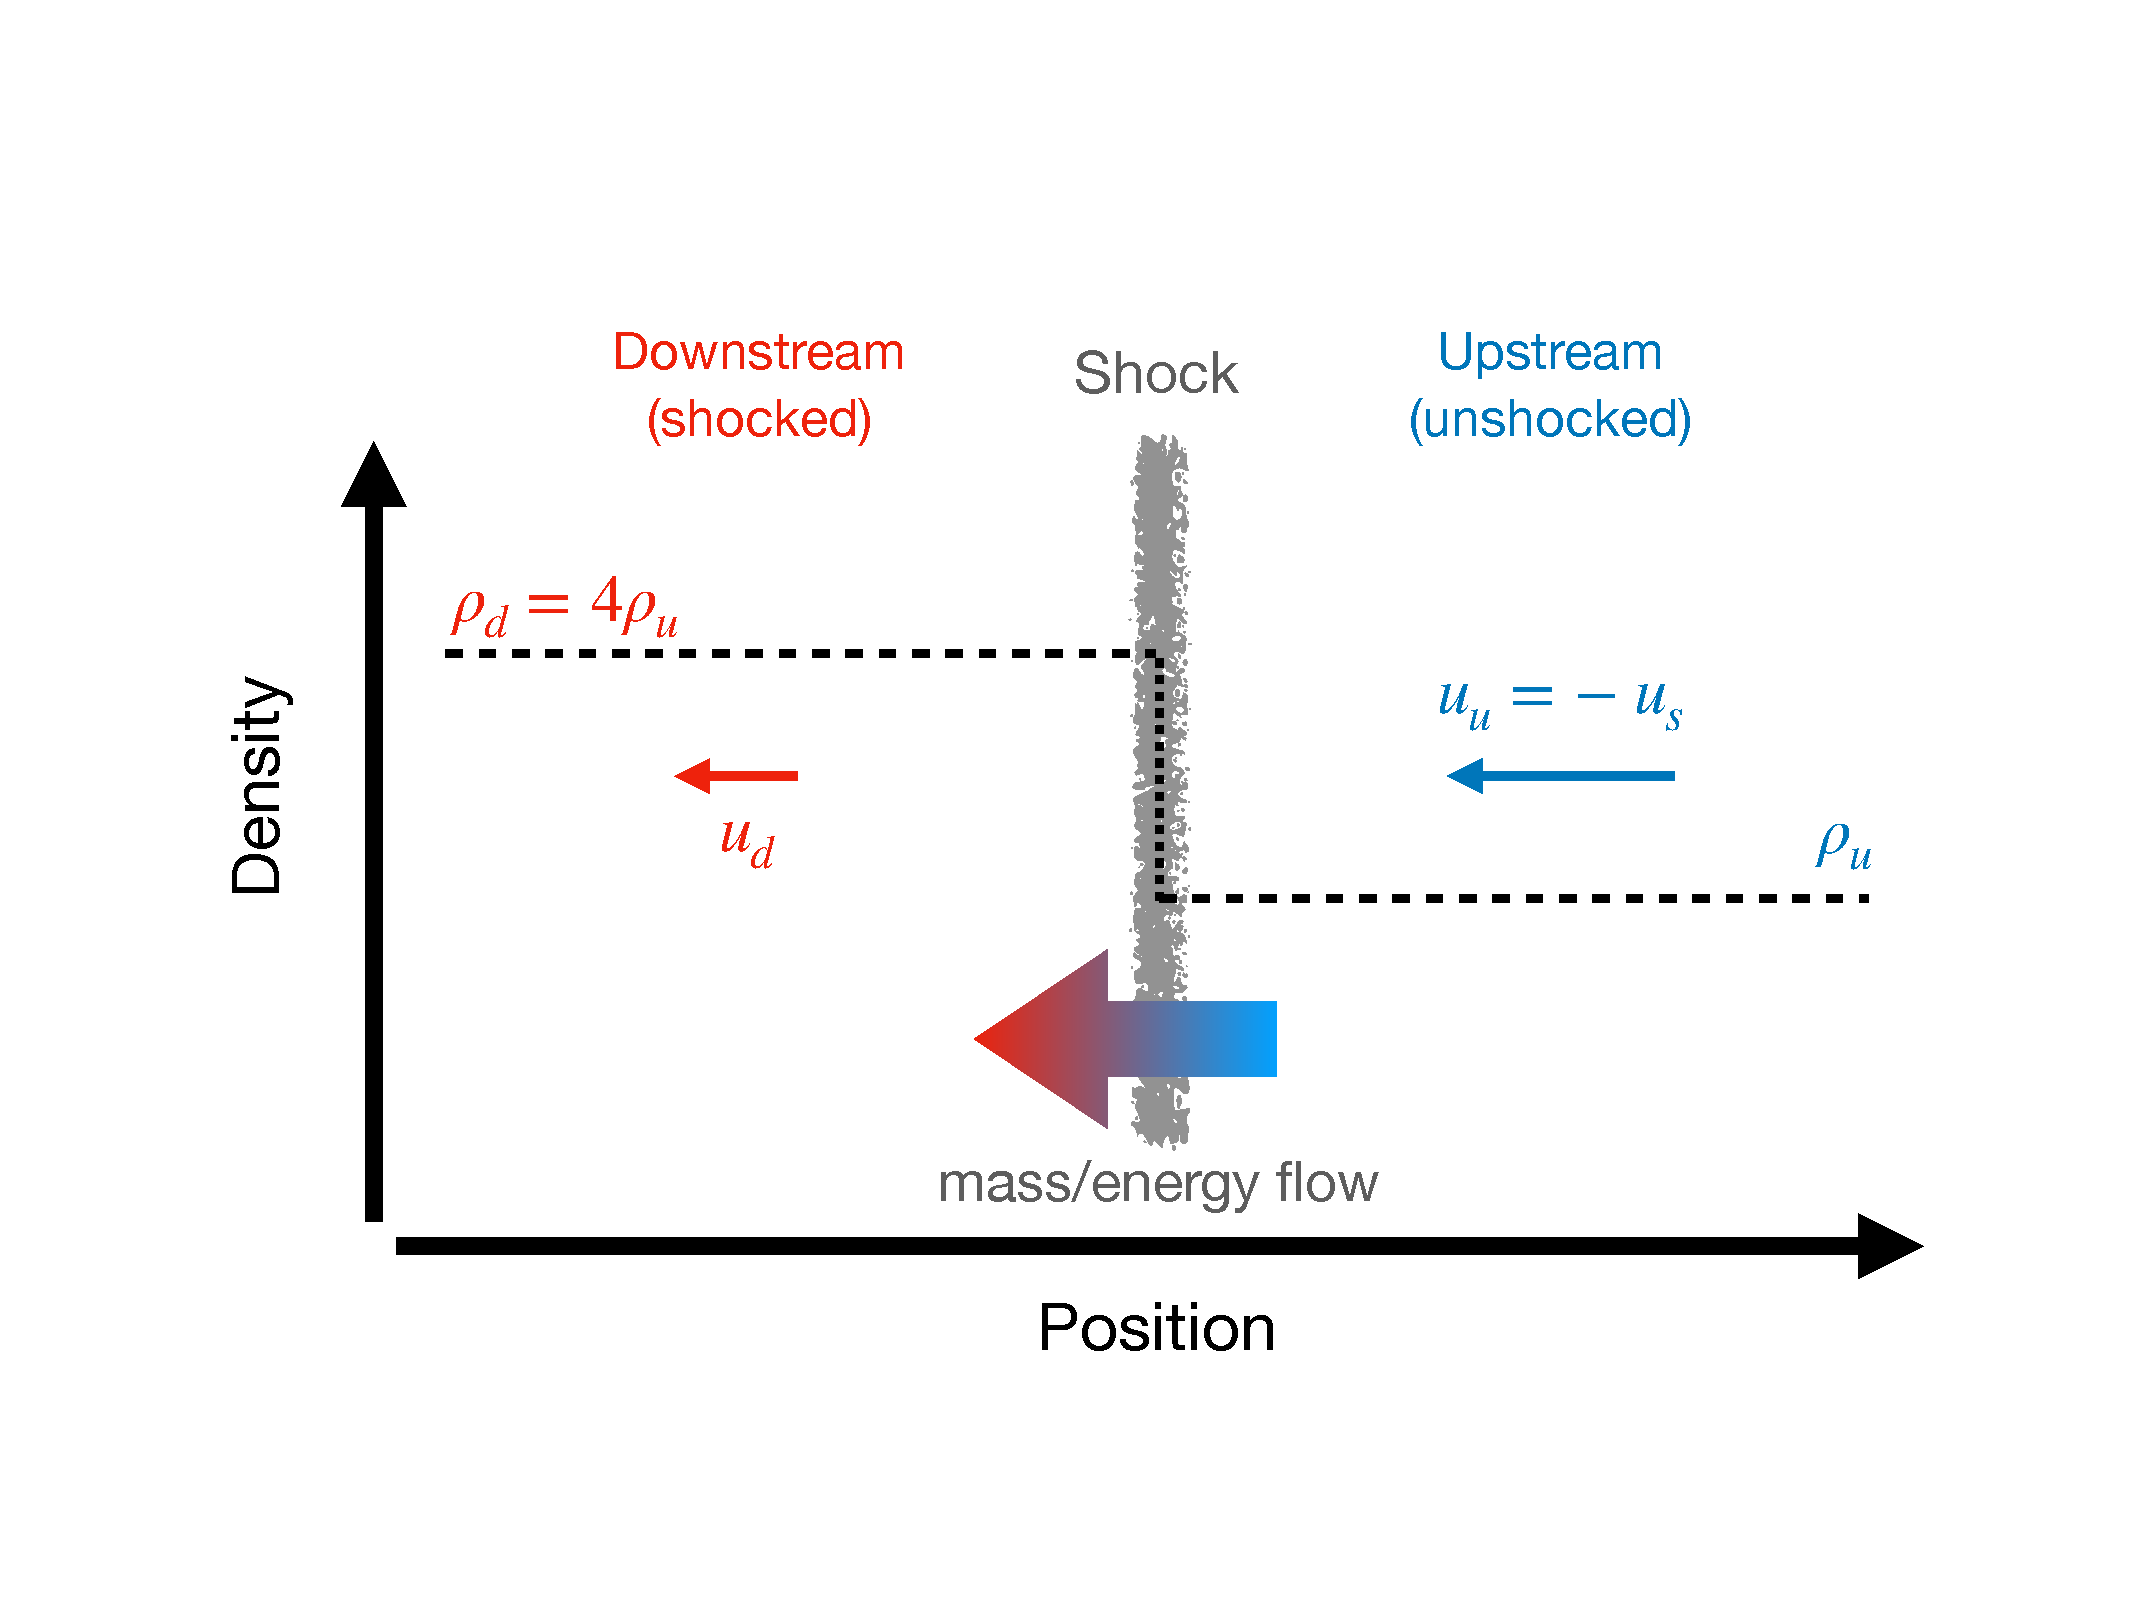
\includegraphics[width=0.57\textwidth]{figures/shockflow.pdf}
\caption{}\label{fig:shockflow}
\end{figure}

In hydrodynamics, solutions often feature \emph{discontinuous} behavior, meaning physical quantities - such as density, pressure, or velocity - can change abruptly across certain surfaces. Mathematically, this manifests as distinct values when approaching the discontinuity from either side. However, in the physical world, these changes are not infinitely sharp as suggested by idealized mathematical models. Instead, the transition occurs over a region that is small relative to all other relevant physical scales.

A \emph{shock} is a particular type of discontinuity characterized by a surface that separates two fluid regions with contrasting properties. Crucially, this surface allows the transfer of mass, momentum, and energy across it (see Figure~\ref{fig:shockflow}). Shocks naturally arise in the non-linear regime of hydrodynamics, including magnetohydrodynamics, as seen in the previous section. 

In astrophysics, shocks are of immense importance because they dramatically alter the physical state of the gas. For instance, post-shock gas often emits significantly more radiation than pre-shock gas, making shocks detectable phenomena.

Astrophysical shocks differ fundamentally from their terrestrial counterparts due to the nature of particle interactions. Under standard atmospheric conditions - where the particle number density is approximately \( n \sim 10^{23} \, \text{cm}^{-3} \) and the collision cross-section is \( \sigma \sim \pi r_A^2 \sim 10^{-16} \, \text{cm}^2 \) (with \( r_A \sim 65 \, \text{pm} \), the atomic radius of nitrogen) - the mean free path of a particle is very short, about \( \lambda \simeq 1 / (n \sigma) \sim 10^{-7} \, \text{cm} \). Frequent collisions in this regime efficiently convert ordered kinetic energy into disordered thermal energy, leading to the formation of a \emph{collisional shock}.

Astrophysical environments, however, present a vastly different picture. Most particles in these regions are ionized, and the cross-sections for interactions between charged particles are orders of magnitude smaller, typically \( \sigma \sim \pi r_0^2 \sim 3 \times 10^{-25} \, \text{cm}^2 \), where \( r_0 \sim 6 \, \text{fm} \) represents the nuclear radius. Additionally, the particle number density in these environments is exceedingly low, around \( n \sim 1 \, \text{cm}^{-3} \). This results in an enormous mean free path, on the order of megaparsecs.

Given these conditions, shocks in astrophysical settings are predominantly \emph{collisionless}. Their formation and energy dissipation mechanisms do not rely on direct particle collisions or Coulomb interactions. Instead, these processes are governed by collective interactions mediated by the ambient magnetic and electric fields, which play a central role in shock dynamics and energy dissipation.

The detailed microphysics of astrophysical shocks are intricate and extend beyond the scope of these lectures. Factors like finite conductivity and plasma instabilities determine the size and structure of the shock transition region. However, despite these complexities at the microscopic level, the conservation laws of mass, momentum, and energy continue to hold and provide a robust framework for understanding shocks at macroscopic scales.

For non-relativistic shock waves, it is helpful to first define a reference frame. In the \emph{Galaxy frame}, the unshocked medium (ISM) is at rest, and the shock propagates through it at a speed \( u^\prime_s \). In this frame, the shocked gas moves at a slower speed, \( u^\prime_d (< u^\prime_s) \), behind the shock front.

However, a more convenient perspective is the \emph{shock front frame}, where the discontinuity surface itself is stationary (\( u_s = 0 \)). In this frame, the upstream medium approaches the shock at a velocity \( u_u = -u^\prime_s \), while the downstream shocked gas recedes from the shock at \( u_d = u^\prime_s - u^\prime_d \). The relative speed between the upstream and downstream fluids is thus \( u_{\text{rel}} = u_d - u_u \). \TODO{check}

Throughout our discussion, we will adopt the shock front frame to simplify calculations and interpretations. In this frame, we categorize physical quantities based on their location relative to the shock. Quantities \emph{upstream} of the shock (before the discontinuity) are labeled with the subscript 'u,' while those \emph{downstream} of the shock (after the discontinuity) are labeled with the subscript 'd.'

In the study of shock dynamics, we focus on key thermodynamic quantities - density, pressure, temperature, and momentum - on either side of the shock (upstream and downstream). To analyze these quantities, we employ conservation equations in the general form \( \frac{dJ}{dz} = 0 \), where \( J \) represents the flux of a conserved quantity, such as mass, energy, or momentum.

This conservation principle implies that the net flux across the shock remains constant. Integrating this over a small region surrounding the shock yields:
%
\[
\int_{-\epsilon}^{\epsilon} \frac{dJ}{dx} \, dx = J_d - J_u = 0,
\]
%
where \( J_d \) and \( J_u \) denote the downstream and upstream fluxes, respectively. To simplify notation, we write this as \( [J]_{\text{sh}} = J_d - J_u = 0 \), emphasizing that there is no net change in the flux across the shock.

Next, we summarize the key conservation equations for a fluid, assuming that the only force acting is the pressure gradient \( \nabla P \), and neglecting effects from magnetic fields or gravity:
%
\begin{itemize}  
\item The equation of mass conservation is given by:
   \begin{equation}
   \frac{\partial \rho}{\partial t} + \nabla \cdot (\rho \vec{u}) = 0~,
   \end{equation}
   where \( \rho \) is the fluid density and \( \vec{u} \) is the velocity field. This ensures that mass is neither created nor destroyed within the system.

\item Conservation of momentum per unit volume is expressed as:
   \begin{equation}
   \rho \frac{\partial \vec{u}}{\partial t} + \rho (\vec{u} \cdot \nabla) \vec{u} = -\nabla P,
   \end{equation}
   which accounts for the balance between inertial forces and pressure gradients in the fluid.

\item The conservation of energy per unit volume can be written as:
   \begin{equation}
   \frac{\partial}{\partial t} \left( \frac{1}{2} \rho u^2 + \rho U \right) + \nabla \cdot \left[ \vec{u} \left( \frac{1}{2} \rho u^2 + \rho U + P \right) \right] = 0,
   \end{equation}
   where \( U \) is the specific internal energy, and \( \epsilon = \rho U \) represents the internal energy per unit volume.
\end{itemize}

\TODO{Why P?}

To simplify the analysis, we focus on a one-dimensional (planar) shock in a steady state (\( \partial_t = 0 \)) within the reference frame where the shock is stationary. 
%
Under these conditions:
\begin{itemize}
\item The mass continuity equation reduces to:
   \begin{equation}
   \frac{\partial}{\partial z} (\rho u) = 0,
   \end{equation}
   indicating that the mass flux \( \rho u \) is constant across the shock.

\item Substituting the mass continuity equation into the momentum equation yields:
\begin{equation}
\rho u \frac{\partial u}{\partial z} = -\frac{\partial P}{\partial z} \quad \rightarrow \quad \frac{\partial}{\partial z} (P + \rho u^2) = 0.
\end{equation}
Here, the total pressure \( P + \rho u^2 \) (comprising gas pressure and the dynamic pressure) is conserved across the shock.

\item Similarly, the energy conservation law in the steady state provides constraints on the total energy flux, incorporating both kinetic and internal energy terms:
%
\begin{equation}
\frac{\partial}{\partial z} \left( \rho u \left[ \frac{1}{2} u^2 + U + \frac{P}{\rho} \right] \right) = 0 
\end{equation}
%
Simplifying further, and expressing the equation in terms of the adiabatic index \( \gamma \) (see Appendix~\ref{app:thermo}), we arrive at:
%
\begin{equation}
\frac{\partial}{\partial z} \left( \frac{1}{2} u^2 + \frac{\gamma}{\gamma - 1}\frac{P}{\rho} \right) = 0 
\end{equation}
\end{itemize}

% in terms of specific enthalpy \( w \) (see Appendix):
%
%\begin{equation}
%w = U + \frac{P}{\rho} = \frac{\gamma}{\gamma - 1}\frac{P}{\rho}
%\end{equation}

To summarize, under the assumption of planar geometry and in the shock frame, the conservation of mass, momentum, and energy fluxes across the shock can be expressed as follows:

\begin{remark}
\begin{eqnarray}
\left[ \rho u \right]_{\rm sh} & = & 0, \label{eq:RH1} \\
\left[ \rho u^2 + P \right]_{\rm sh} & = & 0, \label{eq:RH2} \\
\left[ \frac{1}{2} u^2 + \frac{\gamma}{\gamma - 1} \frac{P}{\rho} \right]_{\rm sh} & = & 0, \label{eq:RH3}
\end{eqnarray}
\end{remark}

These equations are collectively known as the \emph{Rankine-Hugoniot jump conditions}~\cite{}. They serve as the fundamental dynamical equations governing shocks, encapsulating the conservation laws across the discontinuity. Essentially, they establish the relationships between physical quantities - density, pressure, and velocity - on either side of the shock front.

In this framework, we are tasked with solving for three unknowns, corresponding to the post-shock quantities, while having three equations at our disposal. Besides the trivial solution, where all quantities remain unchanged across the shock, our goal is to derive the non-trivial solution that describes the physical changes induced by the shock. This solution characterizes the downstream state in terms of upstream conditions and the properties of the shock.

To proceed, we recall the definition of the sound speed, which is given by:
%
\begin{equation}
c_{\text{s}} = \left( \frac{\partial P}{\partial \rho} \right)^{1/2} = \left(\frac{\gamma P}{\rho}\right)^{1/2}.
\end{equation}

Here, we assume the gas behaves as an ideal gas, with the equation of state \( P = K \rho^\gamma \), where \( \gamma \) is the adiabatic index, or the ratio of specific heats. For a monoatomic gas, in particular, \( \gamma = 5/3 \).

We then introduce the \emph{Mach number}, which quantifies the ratio of the shock speed to the local sound speed in a given region \( i \). This is defined as:
%
\begin{equation}
\mathcal{M}_i = \frac{v_i}{c_{\text{s},i}},
\end{equation}
%
where \( v_i \) is the velocity of the fluid relative to the shock front, and \( c_{\text{s},i} \) is the local sound speed. Using this definition, the momentum flux equation can be expressed as:
%
\begin{equation}
\rho_i u_i^2 + P_i = \rho_i c_{\text{s}, i}^2 \left( \frac{u_i^2}{c_{\text{s},i}^2} \right) + P_i = (1 + \gamma \mathcal{M}_i^2) P_i.
\end{equation}

If we fix the upstream properties \( \rho_u \), \( u_u \), and \( P_u \), the conservation equations (\ref{eq:RH1})-(\ref{eq:RH3}) can be solved to determine the corresponding downstream quantities \( \rho_d \), \( u_d \), and \( P_d \). The solutions are summarized as (see Appendix~\ref{app:RH} for details):
%
\begin{itemize}
\item Density Compression Ratio:  
\begin{equation}
\frac{\rho_d}{\rho_u} = \frac{u_u}{u_d} = \frac{(\gamma + 1) \mathcal{M}_u^2}{(\gamma - 1) \mathcal{M}_u^2 + 2}~.
\end{equation}

\item Pressure Ratio:
\begin{equation}
\frac{P_d}{P_u} = \frac{2\gamma \mathcal{M}_u^2}{\gamma + 1} - \frac{\gamma - 1}{\gamma + 1}~.
\end{equation}

\item Temperature Ratio:
\begin{equation}
\frac{T_d}{T_u} = \frac{\left[ 2\gamma \mathcal{M}_u^2 - (\gamma - 1) \right] \left[ (\gamma - 1) \mathcal{M}_u^2 + 2 \right]}{(\gamma + 1)^2 \mathcal{M}_u^2}~.
\end{equation}
\end{itemize}

Under the assumption of \emph{strong shock conditions}, where \( \mathcal{M}_u \gg 1 \), and considering a monoatomic gas with \( \gamma = 5/3 \), we can derive a simplified expression for the jump in density across the shock:
%
\begin{remark}
\begin{equation}
r = \frac{\rho_d}{\rho_u} = \frac{u_u}{u_d} \, \underset{\mathcal{M} \gg 1}{\longrightarrow} \, \frac{\gamma + 1}{\gamma - 1} \simeq 4,
\end{equation}
\end{remark}
%
where \( r \) represents the \emph{compression factor}.

This result highlights the maximum compression achievable under the conditions of a strong shock, which depends solely on the adiabatic index \( \gamma \). For \( \gamma = 5/3 \), characteristic of a monoatomic gas, the compression factor reaches its theoretical limit of 4. It is important to note that this upper bound arises due to the constraints imposed by the conservation equations and the nature of the ideal gas equation of state.

Similarly, for the pressure jump across the shock, we have:
%
\begin{equation}
\frac{P_d}{P_u} \, \underset{\mathcal{M} \gg 1}{\longrightarrow} \, \frac{2 \gamma}{\gamma + 1} \mathcal{M}_u^2 \simeq \frac{5}{4} \mathcal{M}_u^2.
\end{equation}

This relation shows that the post-shock pressure grows quadratically with the upstream Mach number, indicating that strong shocks are highly efficient at compressing and heating the gas.

In the shock frame, the upstream gas approaches the shock front with velocity \( u_u \), while the downstream velocity \( u_d \) is significantly reduced. For a strong shock with \( \gamma = 5/3 \), the relationship \( u_d \approx \frac{1}{4}u_u \) holds. This deceleration results in an increase in density and pressure as the kinetic energy of the plasma is converted into thermal energy.

However, energy conservation dictates that the kinetic energy lost during the shock transition must transform into \emph{heat}, resulting in a significant increase in the downstream temperature. Examining the temperature ratio \( T_d / T_u \) under strong shock conditions, we find:
%
\begin{equation}
\frac{T_d}{T_u}  \, \underset{\mathcal{M} \gg 1}{\longrightarrow} \, \frac{2 \gamma (\gamma - 1)}{(\gamma +1)^2} \mathcal{M}_u^2.
\end{equation}

By substituting the upstream Mach number \( \mathcal{M}_u^2 = u_u^2 / c_{\text{s},u}^2 \), the downstream temperature can be expressed as:
%
\begin{equation}
k_B T_d = k_B T_u \frac{2 \gamma (\gamma - 1)}{(\gamma + 1)^2} \frac{u_u^2}{c_{\text{s},u}^2}.
\end{equation}

Using the thermodynamic relationships \( c_{\text{s},i}^2 = \gamma P_i / \rho_i \), \( \rho_i = n_i m_p \), and \( P_i = n_i k_B T_i \), into this expression yields:
%
\begin{remark}
\begin{equation}
{\color{red}k_B T_d} = {\color{blue}\frac{3}{16} m_p u_u^2}~.
\end{equation}
\end{remark}

This result demonstrates that \emph{shocks efficiently convert the {\color{blue}bulk kinetic energy of the upstream medium} into {\color{red}thermal (internal) energy in the downstream region}}. 

For typical astrophysical shocks, where upstream velocities \( u_u \gtrsim 10^4 \, \text{km/s} \), the downstream temperature can reach values on the order of \( T_d \sim 10^7 \, \text{K} \). 
%
This heating mechanism explains the radiative signatures - often in the X-ray or higher-energy bands - of shocked plasmas in various astrophysical phenomena.

In summary, as the plasma crosses the shock front, it is:
\begin{remark}
\begin{description}
\item[Compressed:] \( \rho_d = 4 \rho_u \)
\item[Decelerated:] \( v_d = \frac{1}{4} v_u \)
\item[Heated:] \( T_d \ll T_u \)
\end{description}
\end{remark}

The transformation of inflowing kinetic energy into thermal energy in shock waves is inherently tied to the generation of \emph{entropy}. This transformation arises from the dissipation of ordered bulk kinetic energy - where particle velocities are aligned - into disordered internal kinetic energy, or heat. In classical settings, this dissipation is facilitated by particle collisions within the shock wave.
%
However, as previously discussed, the mean free path for collisions in astrophysical environments can be macroscopically large, often exceeding the size of the system. Under such conditions, direct particle collisions become ineffective as a mechanism for energy dissipation. Instead, energy exchange is mediated by \emph{electromagnetic fields}.

In collisionless shocks, the effective thickness of the shock is governed by the scale over which particles interact with the magnetic fields. This scale is typically associated with the \emph{non-relativistic Larmor radius} of a proton.

For a proton with a velocity of \( v \sim 10^4 \, \text{km/s} \) (typical of a supernova explosion) moving within a galactic magnetic field of \( B \sim 1 \, \mu\text{G} \), the Larmor radius \( r_{\text{B}} \) is given by:
%
\[
r_{\text{B}} = \frac{m_p v c}{e B} \simeq 10^{10} \, \text{cm}~.
\]

To put this into perspective, the typical length scales of supernova (SN) explosions are on the order of a parsec. The thickness of the shock layer, characterized by the Larmor radius, is therefore many orders of magnitude smaller than the overall scale of the system. 
%
This vast difference in scales justifies the common approximation in astrophysical modeling that the shock is an \emph{infinitely thin layer}. 

\TODO{entropy}

%The transformation of inflow kinetic energy into thermal energy in shock waves is accompanied by the generation of entropy. The key to this transformation is the collisions among particles within the shock wave. These collisions convert the ordered bulk kinetic energy, where particle velocities are aligned, into disordered internal kinetic energy, or heat.
%
%However, as we have previously noted, the mean free path for collisions in astrophysical conditions can be macroscopically large. In such scenarios, energy exchange among particles is mediated by electromagnetic fields.
%%
%Therefore, the thickness of the shock is more characterized by the non-relativistic Larmor radius of a proton. This radius reflects the scale over which particles are deflected by the magnetic field present at the shock front.
%
%Considering a typical proton velocity of \( \sim 10^4 \) km/s in a supernova explosion, and within a typical galactic magnetic field of \( 1 \mu \)G, the Larmor radius (\( r_{\text{B}} \)) is calculated as:
%%
%\begin{equation}
%r_{\text{B}} = \frac{m_p v c}{e B} \simeq 10^{10}~\text{cm}
%\end{equation}
%
%When compared to typical lengths involved in supernova (SN) explosions, which are on the order of a parsec (see later), the shock thickness is several orders of magnitude smaller. Therefore, in the grand scale of such astrophysical phenomena, the approximation of an infinitely thin shock layer is justified.
%
%Finally, we want to compute the post-shock Mach number \( M_2 \):
%%
%\begin{equation}
%\mathcal M_2 = \frac{u_2}{c_{\rm s,2}} = \mathcal M_1 \frac{u_2}{u_1} \frac{c_1}{c_2} = \mathcal M_1 \frac{u_2}{u_1} \left( \frac{T_1}{T_2} \right)^{1/2}
%\end{equation}
%%
%in the strong shock limit:
%%
%\begin{equation}
%\mathcal M_2 = \mathcal M_1 \frac{\gamma - 1}{\gamma + 1} \left[ \frac{(\gamma + 1)^2}{2\gamma(\gamma - 1) \mathcal M_1^2} \right]^{1/2} = \left( \frac{\gamma - 1}{2\gamma} \right)^{1/2} \simeq 0.45 
%\end{equation}
%%
%so a shock converts supersonic gas into subsonic gas.
%%
%In doing so, it increases the specific entropy of the gas by an amount~(see appendix):
%%
%\begin{equation}
%s_2 - s_1 = c_{\rm P} \ln \left(\frac{T_2}{T_1}\right) - \frac{k}{m} \ln \left( \frac{P_2}{P_1} \right)
%\end{equation}
%%
%In another terminology, a shock changes the entropy shifting gas to a higher adiabat.
%
%Notice then that the non trivial solution makes sense only if the Mach number $M_1$ is larger than one. In the opposite case, we the variation of entropy would be in the sense to decrease it, which is not allowed by second principle of thermodynamics. 
%%
%In other words we would have invented a system to transform heat in ordered work! Shocks can only form in supersonic motion.
%\input{sections/sources/snremnants}
%\newpage

%\chapter{Particle Acceleration}
%\input{sections/acceleration/intro}
%\input{sections/acceleration/generalities}
%\input{sections/acceleration/secondorder}
%\input{sections/acceleration/firstorder}
%\input{sections/acceleration/dsa}
%\input{sections/acceleration/nonlinear}
%\newpage

%\chapter{Particle Transport in Galactic environments}
%\input{sections/transport/grammagepillar}
%\input{sections/transport/solutions}
%\input{sections/transport/implications}
%\newpage

\appendix

%\chapter{Appendix}
%\input{sections/appendix/app_larmor}
%\input{sections/appendix/app_radtransfer}
%\input{sections/appendix/app_intensity}
%% !TEX root = ../..//lectures.tex
\section{Thermodynamics of Adiabatic Processes}
\label{app:thermo}

An \emph{adiabatic process} is characterized by the absence of heat exchange between the system and its surroundings, mathematically expressed as \( \delta Q = 0 \). From the \emph{first law of thermodynamics}, we have:
\begin{equation}
\label{eq:firstlaw}
d\mathcal{U} + P dV = 0,
\end{equation}
where \( \mathcal{U} \) is the internal energy of the system, \( P \) is the pressure, and \( V \) is the volume. This implies that work done by the system (\( P dV \)) must be entirely compensated by a change in its internal energy (\( d\mathcal{U} \)).

For an ideal gas, which follows the equation of state \( P V = n R T \) (\( R \) is the universal gas constant), the internal energy is solely a function of temperature and is given by:
\begin{equation}
\label{eq:nrt}
\mathcal{U} = \alpha n R T = \alpha P V,
\end{equation}
where \( n \) is the number of moles, and \( \alpha = \frac{f}{2} \), with \( f \) being the number of degrees of freedom.

Differentiating \( \mathcal{U} \):
\begin{equation}
\label{eq:dunrdt}
d\mathcal{U} = \alpha n R dT = \alpha (P dV + V dP),
\end{equation}
where we used the ideal gas law to relate \( dT \) to changes in \( P \) and \( V \).

Substituting \( d\mathcal{U} \) from Equation~\ref{eq:dunrdt} into the first law (Equation~\ref{eq:firstlaw}), we get:
\begin{equation}
- P dV = \alpha (P dV + V dP).
\end{equation}
Rearranging terms:
\begin{equation}
-(\alpha + 1) \frac{dV}{V} = \alpha \frac{dP}{P}.
\end{equation}

Integrating both sides:
\begin{equation}
\ln \left( \frac{P}{P_0} \right) = - \frac{\alpha + 1}{\alpha} \ln \left( \frac{V}{V_0} \right),
\end{equation}
or equivalently:
\begin{equation}
P V^{\gamma_g} = \text{constant},
\end{equation}
where \( \gamma_g = \frac{\alpha + 1}{\alpha} = \frac{c_P}{c_V} \) is the \emph{heat capacity ratio}. 
%
This relationship, known as the \emph{polytropic equation}, characterizes a reversible adiabatic process.

\end{document}

#### Ideal Gas Internal Energy
#### Derivation of Adiabatic Condition

#### Internal Energy in Terms of Volume and Pressure
The internal energy for an ideal gas can also be expressed as:
\begin{equation}
\mathcal{U} = n c_V T = \frac{P V}{\gamma_g - 1}.
\end{equation}
Dividing by volume, we get the **internal energy density**:
\begin{equation}
u = \frac{\mathcal{U}}{V} = \frac{P}{\gamma_g - 1}.
\end{equation}

#### Enthalpy and Specific Enthalpy
The **enthalpy** \( \mathcal{H} \) is defined as:
\[
\mathcal{H} = \mathcal{U} + P V.
\]
Dividing by volume, the **enthalpy density** becomes:
\[
\frac{\mathcal{H}}{V} = u + P.
\]

To express enthalpy per unit mass, we introduce the specific internal energy \( \epsilon = \frac{u}{\rho} \), where \( \rho \) is the density. The **specific enthalpy** is:
\begin{equation}
h = \epsilon + \frac{P}{\rho}.
\end{equation}

#### Entropy in Adiabatic Processes
In a reversible adiabatic process, entropy remains constant. The specific entropy \( s \) satisfies:
\[
\frac{\partial s}{\partial t} + \vec{u} \cdot \nabla s = 0.
\]
For a compressible fluid, the conservation of entropy per unit volume (\( \rho s \)) can be expressed as:
\begin{equation}
\frac{\partial (\rho s)}{\partial t} + \nabla \cdot (\rho s \vec{u}) = 0.
\end{equation}

#### Momentum and Energy Conservation
Using the ideal gas law and the specific internal energy:
\[
\epsilon = \frac{1}{\gamma_g - 1} \frac{P}{\rho},
\]
the momentum conservation equation links pressure gradients to the acceleration of the fluid:
\begin{equation}
\frac{\partial \vec{u}}{\partial t} + \vec{u} \cdot \nabla \vec{u} = -\frac{\nabla P}{\rho}.
\end{equation}

---

This version enhances pedagogical clarity by:
1. Explicitly linking each step to physical principles.
2. Clarifying symbols and constants.
3. Highlighting key results with boxed equations.
4. Improving the narrative flow with better transitions and explanatory text.


An adiabatic process is defined by the absence of heat transfer to or from the system \( \delta Q = 0 \). According to the first law of thermodynamics:
\begin{equation}
\label{eq:firstlaw}
d\mathcal U + PdV = 0
\end{equation}
This equation implies that any work (\(PdV\)) performed must be compensated by a change in the internal energy (\(\mathcal U\)), as no heat is exchanged with the surroundings.

For an ideal gas, obeying the equation of state \(PV = nRT\) (where \(R\) is the universal gas constant), the internal energy is given by:
\begin{equation}
\label{eq:nrt} 
\mathcal U = \alpha n R T = \alpha PV 
\end{equation}
Here, \(n\) represents the number of moles, and \( \alpha \) is the number of degrees of freedom divided by 2.

Differentiating Equation~\ref{eq:nrt} results in:
\begin{equation}\label{eq:dunrdt}
d\mathcal U = \alpha n R dT = \alpha (P dV + V dP)
\end{equation}

Substituting this into Equation~\ref{eq:firstlaw} yields:
\begin{equation}
- PdV = \alpha P dV + \alpha V dP \rightarrow -(\alpha + 1) \frac{dV}{V} = \alpha \frac{dP}{P}
\end{equation}

Integrating both sides of this equation, we get:
\begin{equation}
\ln \left( \frac{P}{P_0} \right) = - \frac{\alpha + 1}{\alpha} \ln \left( \frac{V}{V_0} \right) = - \gamma_g \ln \left( \frac{V}{V_0} \right)
\end{equation}
where \( \gamma_g \) is the heat capacity ratio, \( c_V = \alpha R \), and we have used Mayer's relation \(c_P - c_V = R\).

Thus, a reversible adiabatic process (one with no entropy generation) can be characterized by the polytropic process equation:
\begin{remark}
\begin{equation}
PV^\gamma = \text{constant}
\end{equation}
\end{remark}
%%% END CGPT

Notice that for an ideal gas the \emph{internal energy} is solely a function of temperature. Indeed, from Eq.~\ref{eq:nrt}, we obtain 
\begin{equation}
\mathcal U = n c_V T = \frac{PV}{\gamma_g - 1}
\end{equation}

Thus, expressing internal energy per unit volume as \(u\), we get:
%
\begin{equation}
u = \frac{\mathcal U}{V} = \frac{P}{\gamma_g - 1}
\end{equation}

On the other hand, \emph{enthalpy} \( \mathcal H\) is defined as:
\[
\mathcal H = \mathcal U + PV \rightarrow  \frac{\mathcal H}{V} = u + P
\]

Employing the relation \(u = \rho \epsilon\) (where \(\rho\) is the density and \(\epsilon\) is the \emph{specific} internal energy, i.e., energy per unit mass), we derive the \emph{specific} enthalpy:
\begin{remark}
\begin{equation}
h = \frac{1}{\rho} \frac{\mathcal H}{V} = \epsilon + \frac{P}{\rho}
\end{equation}
\end{remark}


%%% END

% Last the first law of thermodynamics states that
% \[
% dU=TdS-PdV
% \]
% with $S$ the entropy,  which is conserved (so $dS=0$).  If we divide by mass we obtain the specific quantities,  namely
% \[
% d\epsilon=-Pd\left(\frac{1}{\rho}  \right)
% \]
%
% Therefore:
% \[
% dw = d\epsilon +\frac{dP}{\rho}+P d\left(\frac{1}{\rho}  \right)=\frac{dP}{\rho}
% \]
%
%
%Noting that $U = \frac{P}{\rho (\gamma − 1)}$ from ideal gas law, with $U$ internal energy per unit mass.
%
%Now introduce the entropy per unit mass $s$,  satisfying the adiabatic condition
%\begin{equation}
%\frac{\partial s}{\partial t} + u \frac{\partial s}{\partial z}=0
%\end{equation}
%Entropy per unit volume would be $\rho s$,  so that we can write (questa si puo derivare ma u e' costante o no?)
%\begin{equation}
%\frac{\partial (\rho s)}{\partial t}+\vec{\nabla}(\rho s\vec{u}) =0 \underset{1d}{\implies} \frac{\partial (\rho s)}{\partial t}+\frac{\partial}{\partial z}(\rho su) =0 
%\end{equation}
%
%The \textbf{enthalpy} of the system is \[ \mathcal W = E + PV \], while the specific enthalpy is \[ w=\epsilon +\frac{P}{\rho} \].
%
%Therefore
%\begin{equation}
%dw=d\epsilon +d\left(\frac{P}{\rho} \right)
%\end{equation}
%On the other hand
%\begin{equation}
%\begin{aligned}
% dE &= dQ-PdV\\
%&=\cancel{TdS} -PdV\\
%\implies d\epsilon &=-Pd\left(\frac{1}{\rho}\right)\\
%&=\frac{P}{\rho^2}d\rho
%\end{aligned}
%\end{equation}
%\begin{equation}
%\implies
%dw=\frac{P}{\rho^2}d\rho +\frac{dP}{\rho}-\frac{P}{\rho^2}d\rho =\frac{dP}{\rho}
%\end{equation}
%Now we can use again the conservation of momentum and write:
%\begin{equation}
%\frac{\partial u}{\partial t}+u\frac{\partial u}{\partial z}=-\frac{\nabla P}{\rho}\equiv \nabla \left[\epsilon +\frac{P}{\rho}  \right]
%\end{equation}
%Remember the energy density per unit volume
%\begin{equation}
%u=\frac{P}{\gamma_g -1}=\rho\epsilon \implies \epsilon =\frac{1}{\gamma_g -1}\frac{P}{\rho}
%\end{equation}
%

%% !TEX root = ../..//lectures.tex
\section{Solving the Rankine-Hugoniot Relations}
\label{app:RH}

The Rankine-Hugoniot relations govern the dynamics of shock waves by connecting the physical quantities across the shock front. In this appendix, we solve the Rankine-Hugoniot relations step by step to illustrate the underlying physics and mathematical structure. The relations are:
%
\begin{eqnarray}
\rho_1 u_1 & = & \rho_2 u_2, \label{eq:mass_conservation} \\
\rho_1 u_1^2 + P_1 & = & \rho_2 u_2^2 + P_2, \label{eq:momentum_conservation} \\
\frac{1}{2} u_1^2 + \frac{\gamma}{\gamma - 1} \frac{P_1}{\rho_1} & = & \frac{1}{2} u_2^2 + \frac{\gamma}{\gamma - 1} \frac{P_2}{\rho_2}. \label{eq:energy_conservation}
\end{eqnarray}

Here, \(\rho\) is the mass density, \(u\) the velocity, \(P\) the pressure, and \(\gamma\) the adiabatic index. The subscripts \(1\) and \(2\) denote the upstream and downstream regions, respectively.

To simplify the energy equation \eqref{eq:energy_conservation}, we normalize it by dividing through by \(\frac{1}{2} u_1^2\):
\begin{equation}
1 + \frac{\gamma}{\gamma - 1} \frac{2 P_1}{u_1^2 \rho_1} = \frac{u_2^2}{u_1^2} + \frac{\gamma}{\gamma - 1} \frac{2 P_2}{u_1^2 \rho_2}.
\end{equation}

Using the momentum conservation equation \eqref{eq:momentum_conservation}, we express \(P_2\):
\begin{equation}
P_2 = P_1 + \rho_1 u_1^2 - \rho_2 u_2^2.
\end{equation}

Introducing the Mach number \(\mathcal{M}_1 = u_1 / c_{\text{s}, 1}\), where \(c_{\text{s}, 1}^2 = \gamma P_1 / \rho_1\), we rewrite the normalized energy equation as:
\begin{equation}
1 + \frac{2}{\gamma - 1} \frac{1}{\mathcal{M}_1^2} = \frac{u_2^2}{u_1^2} \left(1 - \frac{2\gamma}{\gamma - 1} \right) + \left( \frac{2}{\gamma - 1} \frac{1}{\mathcal{M}_1^2} + \frac{2\gamma}{\gamma - 1} \right) \frac{\rho_1}{\rho_2}.
\end{equation}

Defining \( x = u_2 / u_1 \), we obtain:
\begin{equation}
x^2 \mathcal{M}_1^2 (\gamma + 1) - 2x (\gamma \mathcal{M}_1^2 + 1) + 2 + (\gamma - 1) \mathcal{M}_1^2 = 0.
\end{equation}
This quadratic equation yields two solutions: \(x = 1\) (trivial) and the physically relevant:
\begin{equation}
\frac{u_2}{u_1} = \frac{(\gamma - 1) \mathcal{M}_1^2 + 2}{(\gamma + 1) \mathcal{M}_1^2}.
\end{equation}

Returning to the energy equation, we express the pressure ratio as:
\begin{equation}
\frac{P_2}{P_1} = \left[1 + \frac{\mathcal{M}_1^2(\gamma - 1)}{2} \right] \frac{u_1}{u_2} - \frac{\mathcal{M}_1^2(\gamma - 1)}{2} \frac{u_2}{u_1}.
\end{equation}
Substituting \(\frac{u_2}{u_1}\) into this expression, we find:
\begin{equation}
\frac{P_2}{P_1} = \frac{2\gamma \mathcal{M}_1^2}{\gamma + 1} - \frac{\gamma - 1}{\gamma + 1}.
\end{equation}

Using the ideal gas law \(P = \rho R T\), we relate pressure, density, and temperature:
\begin{equation}
\frac{T_2}{T_1} = \frac{P_2}{P_1} \frac{\rho_1}{\rho_2} = \frac{P_2}{P_1} \frac{u_2}{u_1}.
\end{equation}
Substituting the previously derived relations:
\begin{equation}
\frac{T_2}{T_1} = \frac{\left[ 2 \gamma \mathcal{M}_1^2 - (\gamma - 1) \right] \left[ (\gamma - 1) \mathcal{M}_1^2 + 2 \right]}{(\gamma + 1)^2 \mathcal{M}_1^2}.
\end{equation}

The Rankine-Hugoniot relations allow us to determine the downstream physical properties \(u_2, P_2, \rho_2, T_2\) as functions of the upstream Mach number \(\mathcal{M}_1\) and the adiabatic index \(\gamma\). 

%\input{sections/appendix/app_collisions}
%\newpage

% --- Bibliography ---
\bibliography{2024-hea.bib}
\bibliographystyle{myunsrt.bst}

\end{document}
